
Apr\'{e}s avoir d\'{e}finit les acteurs des systémes et les diff\'{e}rentes interactions nous pouvons maintenant définir notre Product Backlog
puis nous pr\'{e}cisions la planification des sprints.

\subsection{Les fonctionnalit\'{e}s du Backlog}
Le Backlog est un art\'{e}fact tr\`{e}s important dans SCRUM. C'est l'ensemble des caract\'{e}ristiques
fonctionnelles ou techniques qui constituent le produit souhait\'{e}.
Nous allons les d\'{e}crire en d\'{e}tails dans le tableau qui suit :



\begin{table}

\begin{tabular}{|l|l|l|}
\hline
Fonctionnalité                                                                                              & Acteur                          & Description                                                                                                                                                     \\
\hline
Gérer un projet                                                                                             & Administrateur                  & \begin{tabular}[c]{@{}l@{}}L’administrateur peut gérer un projet et ses \\tâches correspondantes d’affectation\end{tabular}                                     \\
\hline
Mettre à jour un                                                                                            & \multirow{3}{*}{Administrateur} & \multirow{3}{*}{\begin{tabular}[c]{@{}l@{}}L’administrateur peut changer les détails \\du projet ainsi que l’affectation des membres\\~au projet\end{tabular}}  \\
\cline{1-1}
Projet                                                                                                      &                                 &                                                                                                                                                                 \\
\cline{1-1}
                                                                                                            &                                 &                                                                                                                                                                 \\
\hline
\begin{tabular}[c]{@{}l@{}}Créer ,Modifier ,\\Supprimer un membre\end{tabular}                              & Administrateur                  & \begin{tabular}[c]{@{}l@{}}L’administrateur peut manipuler les données \\des membres\end{tabular}                                                               \\
\hline
\begin{tabular}[c]{@{}l@{}}Créer ,Modifier ,\\Supprimer un client\end{tabular}                              & Administrateur                  & \begin{tabular}[c]{@{}l@{}}L’administrateur peut manipuler les \\données des clients\end{tabular}                                                               \\
\hline
Consulter les rapports                                                                                      & Administrateur                  & L’administrateur peut accéder aux rapports                                                                                                                      \\
\hline
\begin{tabular}[c]{@{}l@{}}Consulter les coordonnées \\des clients sur la carte\\~géographique\end{tabular} & Administrateur                  & \begin{tabular}[c]{@{}l@{}}L’administrateur peut accéder aux \\coordonnées géographiques des clients\end{tabular}                                               \\
\hline
\begin{tabular}[c]{@{}l@{}}Changer l’état et la\\~progression approximative \\de ses tâches\end{tabular}    & Membre                          & \begin{tabular}[c]{@{}l@{}}Le membre peut changer ses taches \\courantes selon l’avancement.\end{tabular}                                                       \\
\hline
\end{tabular}
\centering
\caption{Product Backlog}
\end{table}

\newpage

\subsection{ Planification des sprints}

\FloatBarrier
\begin{table}

\begin{tabular}{|l|l|l|}
\hline
\multirow{2}{*}{Release 1} & Gestion des projets                        & 20 jours  \\
\cline{2-3}
                           & Gestion des membres                        & 7 jours   \\
\hline
\multirow{5}{*}{Release 2} & Gestion des clients                        & 2 jours   \\
\cline{2-3}
                           & Authentification                           & 5 jours   \\
\cline{2-3}
                           & Création des interfaces administrateurs    & 20 jours  \\
\cline{2-3}
                           & Création des interfaces membres            & 5 jours   \\
\cline{2-3}
                           & Modification et design des interfaces~ ~ ~ & 15 jours  \\
\hline
\multirow{2}{*}{Release 3} & Intégration des données                    & 10 jours  \\
\cline{2-3}
                           & Affichage des rapports                     & 7 jours   \\
\hline

\end{tabular}
\centering
\caption{Planification des sprints }
\end{table}
\FloatBarrier


\subsection{Diagramme de Gantt}

\FloatBarrier
\begin{figure}[H]
\center
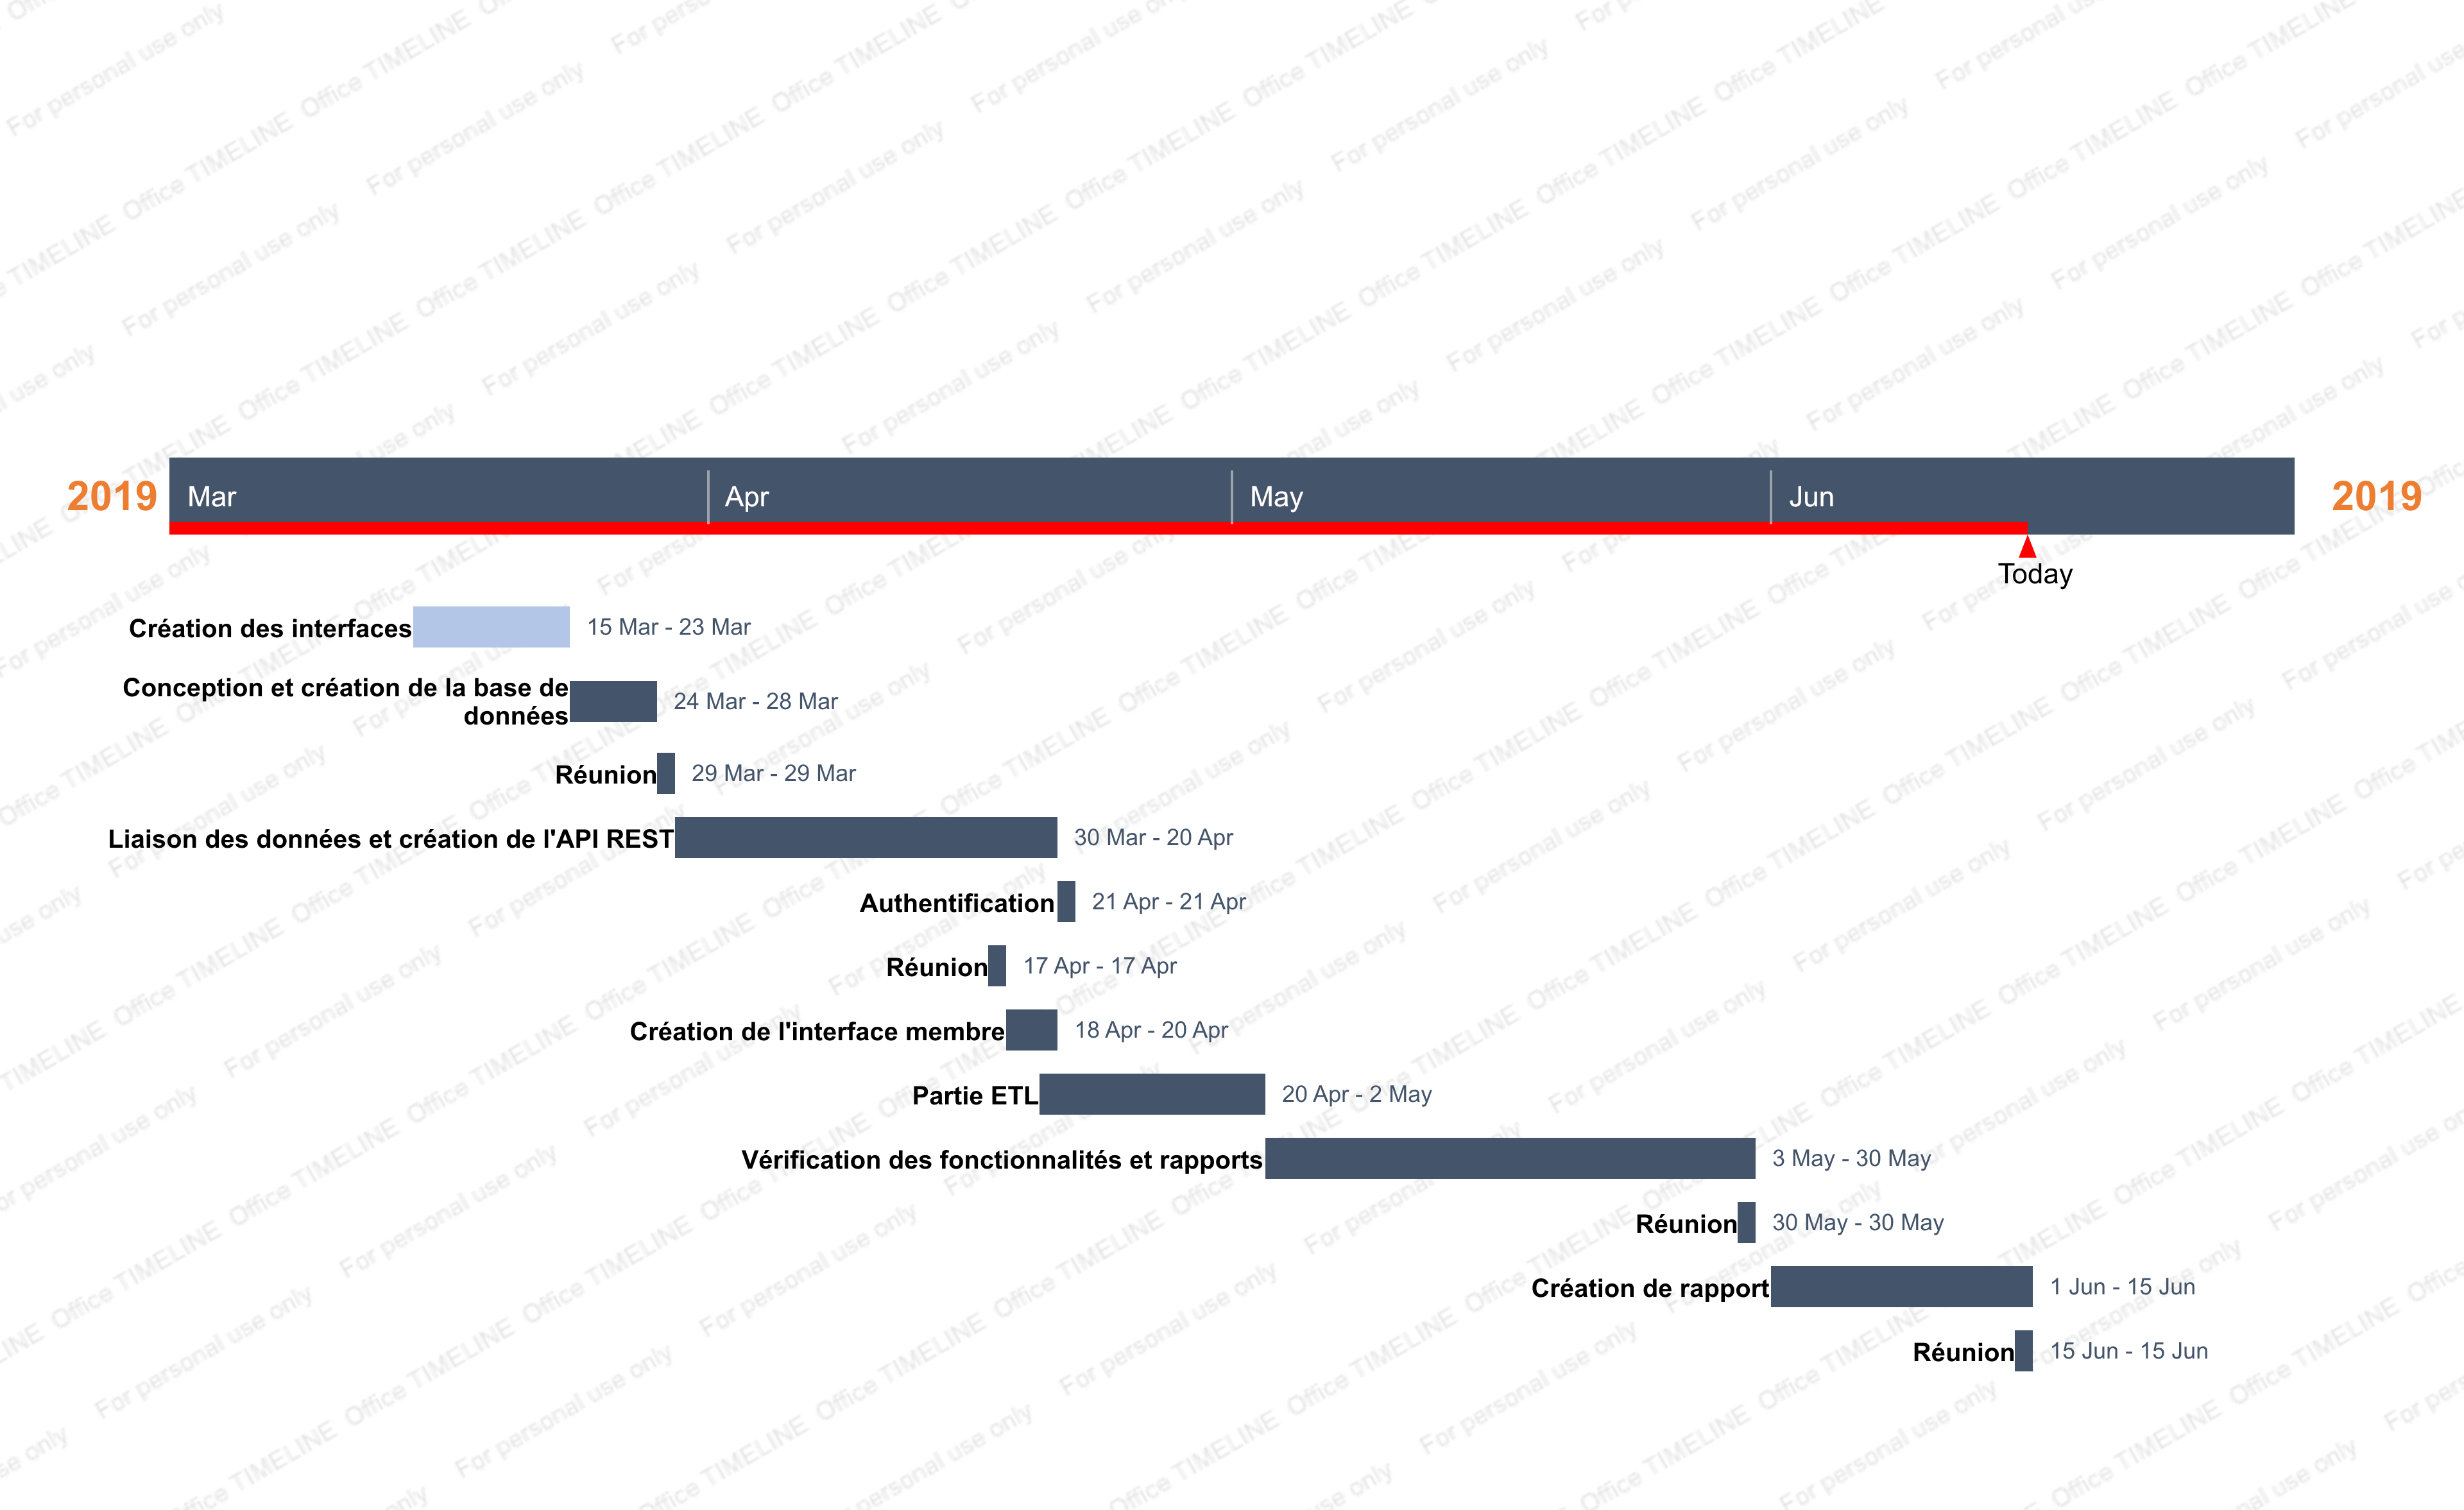
\includegraphics[width=15cm,height=15cm]{./figures/gantt.png}
\caption{Diagramme de Gantt.}
\end {figure}
\FloatBarrier